\section{Dimensionality Reduction}
\thispagestyle{plain}

We are now in the land of unsupervised learning.

\pinkbox{\textbf{Unsupervised Learning Overview\skipthis}: Given only features $\vec{x}$
so a data matrix $\mat{X} \in \mathbb{R}^{N \times p}$, we want to 
find and use structure in the data. Typical unsupervised tasks are
\begin{itemize}
    \item clustering: find groups of similar data points, e.g. similar measurements of solar wind,
    similar pictures, \dots
    \begin{itemize}
        \item \textbf{mean-shift}: group measurements in feature space to modes of their density
        by shifting points to the mean of their neighborhood
        \item \textbf{k-means}: a vector quantizer maps vectors in $\mathbb{R}^p$ to a set of $k$
        centroids, centroids are placed, all vectors are assigned to the nearest centroid, centroids
        are updated to the center of mass of their assigned vectors
        \item \textbf{hierarchical clustering}: start with each point as its own cluster, merge
        clusters (what clusters to merge e.g. based on average distance between their points),
        possibly restricted by connectivity constraints (e.g. by kNN graph)
    \end{itemize}
    \item dimensionality reduction: find a lower-dimensional representation of the data
    \begin{itemize}
        \item \textbf{PCA}: find the directions of maximal variance in the data, the eigenvectors
        of the covariance matrix
        \item approaches retaining local distance information, e.g. \textbf{Multidimensional Scaling (MDS)}
        \item \textbf{Autoencoders}: neural networks that learn to encode and decode data
        \item \textbf{Independent Component Analysis (ICA)}: decomposition of a signal into independent non-Gaussian sources
    \end{itemize}
    \item density estimation: estimate the probability density function of the data (e.g. histograms, kernel density estimation)
\end{itemize}
}

Consider we have measured data $\vec{x}_1, \dots, \vec{x}_N \in \mathbb{R}^p$ which we collect into
a data matrix $\mat{X} \in \mathbb{R}^{N \times p}$. Our measurements might not reflect the true
dimensionality of our data / some dimensions might not be as informative as others. Consider
for instance we capture movement by multiple cameras - each camera captures millions
of pixels (each e.g. a greyscale dimension), but the intrinsic dimensionality of the movement
is much lower (e.g. maximally 3D). Simple examples in 1D and 2D can be found in figure \ref{fig:dimred}.

\begin{figure}

    \centering
    \begin{subfigure}{0.55\textwidth}
      \centering
      \includesvg[width=.95\linewidth]{figures/dimred12.svg}
      \caption{2D data with 1 relevant dimension.}
      \label{fig:dimred1}
    \end{subfigure}%

    \begin{subfigure}{0.75\textwidth}
        \centering
        \includesvg[width=.95\linewidth]{figures/swiss_roll.svg}
        \caption{3D data with 2 relevant dimensions.}
        \label{fig:dimred2}
      \end{subfigure}

    \caption{Simple examples of data with lower intrinsic dimensionality.}
    \label{fig:dimred}

\end{figure}

\bluebox{\textbf{Aim:} Given $\mat{X} \in \mathbb{R}^{N \times p}$, we want to find a lower-dimensional
representation $\mat{Z} \in \mathbb{R}^{N \times q}$ with $q < p$ still capturing the (main)
structure of the data. We project onto lower-dimensional \textbf{latent-manifolds}. Latent
variables can only be inferred indirectly from our observed variables and might correspond
to aspects of physical reality (e.g. our 1d movement captured by the cameras). In the latent
space items resembling each other are closer together.\footnote{Note that e.g. the latent
space of a machine learning model might be completely unintuitive.}}

Applications of dimensionality reduction include
\begin{itemize}
    \item visualization of high-dimensional data
    \item lossy data compression
    \item speed-up of learning algorithms
    \item noise reduction
\end{itemize}

\subsection{Principal Component Analysis (PCA)}
In PCA we \textbf{linearly} transform the dataset into a new coordinate system such that
most of the variation in the data is captured by the lower dimensions.

The principal components are an orthonormal basis, with the first principal component
being along the direction of the most variance and so on.

An example of PCA applied to a 2D dataset is shown in figure \ref{fig:pca}.

\begin{figure}[!htb]
    \centering
    \includesvg[width=.75\textwidth]{figures/pca_example.svg}
    \caption{PCA applied to a 2D dataset.}
    \label{fig:pca}
\end{figure}

\subsubsection{Deriving the principal components from finding the direction with maximum variance}
\note{One should mean-center the features before applying PCA - it is a linear transformation. We set
$\mat{X}$ to
\begin{equation}
    \mat{X} = \mat{X} - \underset{N\times 1}{\vec{1}} \vec{\mu}^T, \quad \text{means of features } \vec{\mu} \in \mathbb{R}^p
\end{equation}
so the covariance matrix
\begin{equation}
    \mat{S} = \frac{1}{N} \left( \mat{X} - \underset{N\times 1}{\vec{1}} \vec{\mu}^T \right)^T \left( \mat{X} - \underset{N\times 1}{\vec{1}} \vec{\mu}^T \right) = \frac{1}{N} \mat{X}^T \mat{X}
\end{equation}
}

The first principal component is given by the direction with maximum (sample) variance
\begin{equation}
    \vec{v}^* = \argmax_{\vec{v}, ||\vec{v}|| = 1} \Var(\mat{X}\vec{v}) = \argmax_{\vec{v}, ||\vec{v}|| = 1} \frac{1}{N} \sum_{i=1}^{N} (\vec{x}_i^T \vec{v})^2 = \argmax_{\vec{v}, ||\vec{v}|| = 1} \vec{v}^T \mat{S} \vec{v}
\end{equation}

We can formulate this as the optimization problem
\begin{equation}
    \vec{v}^* = \argmax_{\vec{v}} \left\{ \underbrace{\vec{v}^T \mat{S} \vec{v} - \lambda (\vec{v}^T \vec{v} - 1)}_{:=\,\mathcal{L}(\vec{v},\lambda)} \right\}
\end{equation}
where $\lambda$ is a Lagrange multiplier to include the condition $||\vec{v}|| = 1$ ($\partial_{\lambda} \mathcal{L} = 0
\rightarrow \vec{v}^T \vec{v} = 1$).

Then
\begin{equation}
    \partial_{\vec{v}} \mathcal{L} = 2 \mat{S} \vec{v} - 2 \lambda \vec{v} = 0 \rightarrow \mat{S} \vec{v} = \lambda \vec{v}
\end{equation}
where multiplying by $\vec{v}^T$ from the left and using $\vec{v}^T \vec{v} = 1$ gives
\begin{equation}
    \vec{v}^T \mat{S} \vec{v} = \Var(\mat{X}\vec{v}) = \lambda
\end{equation}

\greenbox{So the direction of maximum variance is the eigenvector with the largest eigenvalues $\lambda_{\text{map}}$.}

\note{An alternative perspective is finding the directions to which all points in the dataset have the lowest
squared distance (different from Linear Regression as here an orthogonal distance is minimized).}

\subsubsubsection{The principal components and dimensionality reduction}
The principal components are the eigenvectors of the covariance matrix
(here assuming mean-centered data)
\begin{equation}
    \mat{S} = \frac{1}{N} \mat{X}^T \mat{X} \text{ symmetric, real, positive semi-definite } (\vec{u}^T \mat{S} \vec{u} \geq 0 \forall \vec{u})
\end{equation}
so $S$ has only real non-negative eigenvalues and the eigenvectors form an orthonormal basis
(symmetric matrices are diagonalizable, EVs of real symmetric matrices are orthogonal) - our principal
components.

\greenbox{PCA rotates the data so that it becomes variance-aligned.}

We project to lower dimensions by projecting our data onto the principal components.

\bluebox{\textbf{How many principal components to keep?} One can look at the explained variance
via the eigenvalues and plot them, as illustrated in figure \ref{fig:explained_variance}.}

\begin{figure}
    \centering
    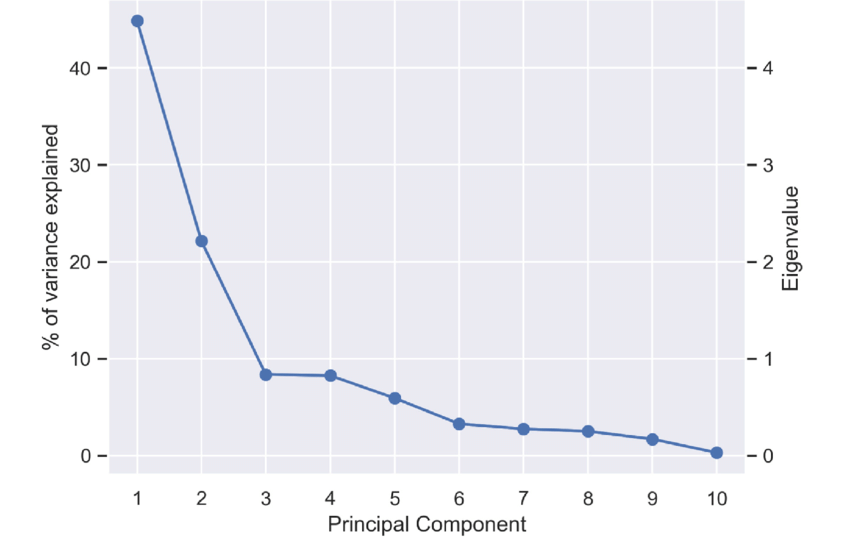
\includegraphics[width=.75\textwidth]{figures/var_exp.png}
    \caption{Explained variance of the principal components (scree plot).}
    \label{fig:explained_variance}
\end{figure}

\subsection{Nonlinear Dimensionality Reduction I: Nonlinear PCA}
\problem{PCA is a linear transformation, it will not be able to reduce non-linear structures
to lower dimensions, as illustrated in figure \ref{fig:pca_examples}.}

\begin{figure}[!htb]
    \centering
    \includesvg[width=.95\textwidth]{figures/PCA.svg}
    \caption{PCA applied to data with non-linear structure.}
    \label{fig:pca_examples}
\end{figure}

\idea{Map the data to a higher dimensional space, where the structure might become reducible
to lower dimensions by a linear transformation, see figure \ref{fig:nonlinear_pca}.}

\begin{figure}[!htb]
    \centering
    \includesvg[width=.95\textwidth]{figures/KernelPCA.svg}
    \caption{Nonlinear PCA (Kernel PCA) applied to data with non-linear structure.}
    \label{fig:nonlinear_pca}
\end{figure}

As before we do a transformation to a higher dimensional space by

\begin{equation}
    \vec{\phi} : \mathbb{R}^p \rightarrow \mathbb{R}^q, \quad q > p
\end{equation}

where our aim is not to directly use such a transformation, but to 
replace the scalar product in this high-dimensional space by a kernel function

\begin{equation}
    k(\vec{x}_i, \vec{x}_j) = \vec{\phi}(\vec{x}_i)^T \vec{\phi}(\vec{x}_j)
\end{equation}

\subsubsection{Kernel PCA}
Our principal components in the high-dimensional space are the eigenvectors of the covariance
matrix
\begin{equation}
    \mat{S} = \frac{1}{N} \left( \mat{\Phi} - \underset{N\times 1}{\vec{1}} \vec{\bar{\Phi}}^T \right)^T \left( \mat{\Phi} - \underset{N\times 1}{\vec{1}} \vec{\bar{\Phi}}^T \right) \in \mathbb{R}^{q \times q}
\end{equation}

\note{While $\mat{X}$ might have centered features, we still to center the features in $\mat{\Phi}$.
We will later do this in the kernel, for now assume $\mat{\tilde{\Phi}}$ to have centered features.}

\subsubsubsection{Finding a formulation where the projection to the principal components is only expressed in terms
of a kernel function}
\problem{The covariance matrix is $q\times q$ but we want to go very high dimensional, and this only 
implicitly by the kernel function. The eigenvectors will also be $\in \mathbb{R}^q$ - we will never
explicitly be able to compute them. We never explicitly operate in the high-dimensional space.}

\idea{What if we could instead somehow use the eigenvalues and -vectors
of the Gram matrix $\mat{\tilde{\Phi}} \mat{\tilde{\Phi}}^T \in \mathbb{R}^{N \times N}$
to formulate the projection onto the principal components?}

Consider the eigenvectors of the Gram matrix
\begin{equation}
    \frac{1}{N} \mat{\tilde{\Phi}} \mat{\tilde{\Phi}}^T \vec{u} = \lambda \vec{u}, \quad \vec{u} \in \mathbb{R}^N
\end{equation}
and multiply from the left with $\mat{\tilde{\Phi}}^T$

\begin{equation}
    \frac{1}{N} \mat{\tilde{\Phi}}^T \mat{\tilde{\Phi}} \left( \mat{\tilde{\Phi}}^T \vec{u} \right) = \lambda \left( \mat{\tilde{\Phi}}^T \vec{u} \right)
\end{equation}

Then we see that $\vec{v} = \mat{\tilde{\Phi}}^T \vec{u}$ is an eigenvector of the covariance matrix to the same eigenvalue
(not of unit length though). We can find the normalization by
\begin{equation}
    ||\vec{v}||^2 = \vec{v}^T \vec{v} = \vec{u}^T \mat{\tilde{\Phi}} \mat{\tilde{\Phi}}^T \vec{u} = N \lambda ||\vec{u}||^2
\end{equation}
so if $\vec{u}$ is a normalized eigenvector of the Gram matrix $\mat{G} = \frac{1}{N} \mat{\tilde{\Phi}} \mat{\tilde{\Phi}}^T$
\begin{equation}
    \vec{v} = \frac{1}{\sqrt{N \lambda}} \mat{\tilde{\Phi}}^T \vec{u} = \frac{1}{\sqrt{N \lambda}} \sum_{i = 1}^{N} u_i \vec{\phi}_{\vec{x}_i}
\end{equation}
is a normalized eigenvector of the covariance matrix $\mat{S} = \frac{1}{N} \mat{\tilde{\Phi}}^T \mat{\tilde{\Phi}}$.

\greenbox{So given a vector $\vec{x}_j \in \mathbb{R}^p$ and its high dimensional representation $\vec{\phi}_{\vec{x}_j} \in \mathbb{R}^q$
(which will not be necessary explicitly), we get the projection on a principal component
\begin{equation}
    \vec{\tilde{\phi}}_{\vec{x}_j}^T \vec{v} = \frac{1}{\sqrt{N \lambda}} \sum_{i = 1}^{N} u_i \vec{\tilde{\phi}}_{\vec{x}_j}^T \vec{\tilde{\phi}}_{\vec{x}_i} = \frac{1}{\sqrt{N \lambda}} \sum_{i = 1}^{N} u_i \tilde{k}(\vec{x}_i,\vec{x}_j)
\end{equation}
where $\vec{u} \in \mathbb{R}^N$ is the eigenvector of the Gram matrix $\mat{G} = \frac{1}{N} \mat{\tilde{\Phi}} \mat{\tilde{\Phi}}^T \in \mathbb{R}^{N \times N}$
with
\begin{equation}
    G_{ij} = \frac{1}{N} \tilde{k}(\vec{x}_i,\vec{x}_j)
\end{equation}
to the eigenvalue $\lambda$ (largest eigenvalue for first principal component).}

\textbf{We therefore have a formulation of the projection to the principal components of a kernelized PCA only in terms of kernel expressions.}

\subsubsubsection{Kernel expression for mean centered projected features}
What's now left to do is to find an expression for
\begin{equation}
    \tilde{k}(\vec{x}_i,\vec{x}_j) = \vec{\tilde{\phi}}_{\vec{x}_i}^T \vec{\tilde{\phi}}_{\vec{x}_j}
\end{equation}
for the mean centered features
\begin{equation}
    \vec{\tilde{\phi}}_{\vec{x}_i} = \vec{\phi}_{\vec{x}_i} - \frac{1}{N} \sum_{k=1}^{N} \vec{\phi}_{\vec{x}_k}
\end{equation}
so
\begin{equation}
    \begin{aligned}
        \tilde{k}(\vec{x}_i,\vec{x}_j) &= \vec{\tilde{\phi}}_{\vec{x}_i}^T \vec{\tilde{\phi}}_{\vec{x}_j} \\
                                       &= \underbrace{\vec{\phi}_{\vec{x}_i}^T \vec{\phi}_{\vec{x}_j}}_{:=k(\vec{x}_i,\vec{x}_j)} \\
                                       &- \frac{1}{N} \sum_{k=1}^{N} \underbrace{\vec{\phi}_{\vec{x}_i}^T \vec{\phi}_{\vec{x}_k}}_{:=k(\vec{x}_i,\vec{x}_k)}\\
                                       &- \frac{1}{N} \sum_{k=1}^{N} \underbrace{\vec{\phi}_{\vec{x}_k}^T \vec{\phi}_{\vec{x}_j}}_{:=k(\vec{x}_k,\vec{x}_j)} \\
                                       &+ \frac{1}{N^2} \sum_{k=1}^{N} \sum_{l=1}^{N} \underbrace{\vec{\phi}_{\vec{x}_k}^T \vec{\phi}_{\vec{x}_l}}_{:=k(\vec{x}_k,\vec{x}_l)}
    \end{aligned}
\end{equation}
so we have found an expression just in terms of the kernel function, e.g. with
the RBF (radial basis function) kernel
\begin{equation}
    k(\vec{x}_i, \vec{x}_j) = \exp\left( - \frac{||\vec{x}_i - \vec{x}_j||^2}{2\sigma^2} \right), \quad \text{free parameter } \sigma
\end{equation}

\subsection{Nonlinear Dimensionality Reduction II: Further techniques}
\subsubsection{Linear discriminant analysis for dimensionality reduction of classified data}
Here we find directions better separating groups. One
approach is to calculate the in-between-class and
withing-class scatter matrices for all classes and
use the eigenvectors of them, sorted by the eigenvalues
as \textit{principal components}, akin to PCA.

\subsubsection{Retaining (local) distance information or neighbor structure}
Consider high dimensional samples $\vec{x}_i \in \mathbb{R}^{p^*}$ with distances
\begin{equation}
    d_{ij}^* = ||\vec{x}_i - \vec{x}_j||^2
\end{equation}
\bluebox{\textbf{Aim:} Find a low dimensional embedding $\vec{z}_i \in \mathbb{R}^p$ with $p < p^*$ such that
with distances $d_{ij} = ||\vec{z}_i - \vec{z}_j||^2$ that distance information is preserved.}

\subsubsubsection{Global preservation of distance information}
In this approach, we choose the set $\{ z_i \}$ such that

\begin{equation}
    \{ z_i \} = \argmin_{\{ z_i \}} \sum_i \sum_j M(d_{ij}, d^*_{ij})
\end{equation}

with $M$ being a metric comparing distances, for instance

\begin{equation}
    M_{\text{MDS,Kruskal}} = (d_{ij} - d^*_{ij})^2, \quad M_{\text{MDS,Sammon}} = \frac{(d_{ij} - d^*_{ij})^2}{d^*_{ij}}
\end{equation}

where \textbf{MDS} stands for \textbf{Multidimensional Scaling} - a specific
dimensionality reduction technique.

\note{Kernel PCA with Gaussian kernel and MDS with Kruskal metric are equivalent.
\begin{equation}
    \sum_i \sum_j (d_{ij} - d^*_{ij})^2
\end{equation}
is minimized when the data matrix is projected onto the kernelized principal components.
}

\subsubsubsection{Local preservation of distance information}
We follow the steps
\begin{enumerate}
    \item Construct a symmetric k-nearest-neighbor-graph (KNNG)
    \pinkbox{\textbf{Intermezzo: K-nearest-neighbor-graph}: In the KNNG $\vec{x}_i$
    is connected to $\vec{x}_j$ if $\vec{x}_j$ is among the $k$ nearest neighbors of $\vec{x}_i$ among
    all points in the dataset. Note that while $\vec{x}_j$ might be in the k-nearest neighbor list
    of $\vec{x}_i$, $\vec{x}_i$ might not be in the k-nearest neighbor list of $\vec{x}_j$. In a 
    symmetric KNNG, we ignore this directionality, two points are connected if one if in the
    nearest neighbor list of the other.}
    \item We phrase the preservation of local structure as a potential problem
    \begin{enumerate}
        \item if $\vec{x}_i$ and $\vec{x}_j$ are symmetric neighbors, an attractive
        potential is assigned to $\vec{z}_i$ and $\vec{z}_j$
        \item a weak repulsion is assigned to all pairs $\vec{z}_i$ and $\vec{z}_j$
        ($\mathcal{O}(N^2)$ repulsion terms)
    \end{enumerate}
    \item Minimize the potential starting from e.g. random $\vec{z}_i$
\end{enumerate}

Based on different potentials, different techniques are derived, 
as illustrated in figure \ref{fig:distance_retaining_approaches}.

\begin{figure}[!htb]
    \centering
    \includesvg[width=.95\textwidth]{figures/distance_retaining_approaches.svg}
    \caption{Different approaches to retain distance information.}
    \label{fig:distance_retaining_approaches}
\end{figure}

\subsubsubsection{Isomap - distance preservation along geodesics}
\redbox{\textbf{Problem of MDS}: Euclidian distances in the original space might
not best represent the true distances in the data.}

\idea{Preserve distance information along the geodesics of the data, approximated by shortest paths
between points on the K-nearest-neighbor-graph ($\rightarrow$ Djikstra algorithm). Then apply MDS to the geodesic distances.}

This is illustrated in figure \ref{fig:isomap}.

\begin{figure}[!htb]
    \centering
    \includesvg[width=.95\textwidth]{figures/isomap.svg}
    \caption{Isomap applied to data with non-linear structure.}
    \label{fig:isomap}
\end{figure}

\subsubsubsection{Locally Linear Embedding (LLE)}
\begin{enumerate}
    \item A set of nearest neighbors is found as each point
    \item As set of weights is computed that describes the point as a linear combination of its neighbors
    \item a low dimensional embedding is found such that a point is still described with the same weighted linear combination of its neighbors
\end{enumerate}

\subsubsubsection{t-SNE (t-distributed stochastic neighbor embedding)}
\begin{itemize}
    \item construct a probability distribution over pairs of the high-dimensional data points,
    such that similar objects have higher probabilities
    \item a similar low dimensional probability distribution is constructed
    and the Kullback-Leibler divergence\footnote{\begin{equation}
        D_{\mathrm{KL}}(P \| Q)=\sum_{x \in \mathcal{X}} P(x) \log \left(\frac{P(x)}{Q(x)}\right)
        \end{equation}} (relative entropy) between the two distributions is minimized
\end{itemize}

\subsubsection{Autoencoders}
\idea{Train a neural network to compress and decompress the data - extraction
at the compressed layer is the low-dimensional representation.}

An autoencoder is illustrated in figure \ref{fig:autoencoder}.

\begin{figure}[!htb]
    \centering
    \includesvg[width=.95\textwidth]{figures/autoencoder.svg}
    \caption{Autoencoder.}
    \label{fig:autoencoder}
\end{figure}

The loss used in training is

\begin{equation}
    \mathcal{L} = \sum_i^N ||\vec{x}_i - \vec{\tilde{x}}_i||^2
\end{equation}

\pagebreak